\subsection{Calculation of the charge carriers drift velocities}
\label{sec:drift}

\subsubsection{Introduction}
\label{sec:drin}
Following a $\gamma$-ray interaction, the produced electron-hole pairs
will separated and start to drift under the influence of the
electrostatic field produced by the potential applied on the detector
electrodes. One can define the mobility $\mu_{e,h}$ of the electrons
$e$ and holes $h$ as the variable which gives the relation between the
electric field $\mathbf{E}(\mathbf{r})$ and the drift velocity
\begin{equation}
  \label{eq:mobi}
  \mathbf{v}(\mathbf{r}) = \mu_{e,h} \mathbf{E}(\mathbf{r}),
\end{equation}
where $\mathbf{r}$ indicates the position. $\mu_{e,h}$ depend on the
temperature, the electric field and the structure of the germanium
crystal. As long as the electron and hole temperatures do not differ
much from the lattice temperature, the drift velocity is proportional
to the electrical field and the lattice orientation has no influence.
In this case the mobility can be simplified to just a number
$\mu_{e,h} = \mu_{0}$. In germanium detectors cooled at liquid
nitrogen temperature the electron/hole pairs are hotter than the
lattice. The drift velocity in this condition is influenced by the
crystal lattice orientation and not always parallel to the applied
electrical field.

Germanium has the same crystalline structure as silicon and diamond, namely, a face-centered cubic (FCC) structure, in which each atom lies at the center of a regular tetrahedron, and is surrounded at its apices by four atoms as shown in Fig.~\ref{fig:xtal}
\begin{figure}[tbhp]
  \centering
  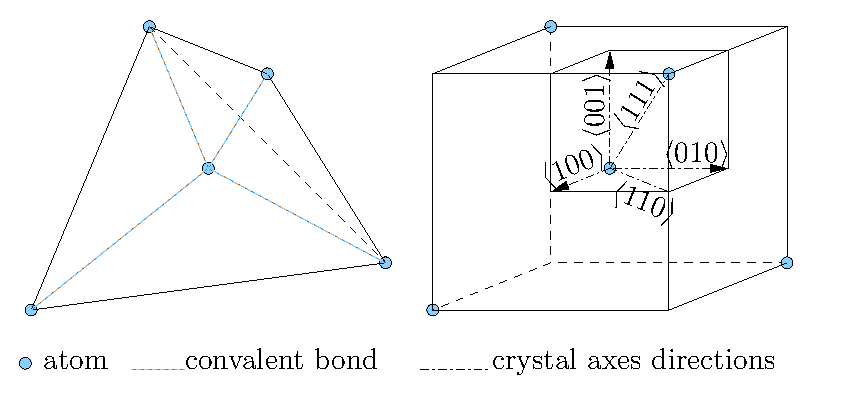
\includegraphics[width=0.6\textwidth]{xtalStruc.eps}  
  \caption{Structure of germanium crystal.}
  \label{fig:xtal}
\end{figure}

Due to the crystal lattice symmetry in germanium, in three directions, the crystallographic $\langle100\rangle$, $\langle110\rangle$ and $\langle111\rangle$, the mobility always has to be aligned with the electrical field. Consequently, the drift velocity has to be aligned with the symmetry axis. Therefore we can obtain not transverse anisotropy but longitudinal anisotropy of the drift mobility. Experimental data on the longitudinal anisotropy in these specific directions can be found in literature. The mobility data can be well fitted in any principal crystallographic direction with the parameterization:
\begin{equation}
  \label{eq:para}
  v = \frac{\mu_{0}E}{[1+(\frac{E}{E_{0}})^{\beta}]^{1/\beta}} -   \mu_{n}E
\end{equation}
At low fields, the mobility becomes isotropic and therefore the mobility fit parameter $\mu_{0}$ is expected to become independent of the crystallographic direction. For hot electrons, the departure from a linear $v \sim E$ relation is modeled through the parameters $E_{0}$ and $\beta$. At high field, Mihailescu \textit{et al.}~\cite{miha} have added the term $\mu_{n}E$ to account for the \emph{Gunn effect} that was observed by Ottaviani \textit{et al.}~\cite{otta} for field strengths above 3~kV$/$cm at 80~K. However, this effect is insignificant in our detector operated with field strengths 0.1-3~kV$/$cm. Parameterization values fitted with the experimental data are summarized in Table~\ref{tab:pars}. The values from two different references are quite different from each other. We'd better measure it by ourselves again.

\begin{table}[tbhp]
  \centering
  \begin{tabular}{ccccccc}\hline\hline
     Reference & Carrier & Direction & $\mu_{0} \left[ \frac{\mbox{cm}^{2}}{\mbox{V}\cdot\mbox{s}} \right]$ & $E_{0} \left[ \frac{\mbox{V}}{\mbox{cm}} \right]$ & $\beta$ & $\mu_{n} \left[ \frac{\mbox{cm}^{2}}{\mbox{V}\cdot\mbox{s}} \right]$ \\\hline
& Electron & $\langle111\rangle$ & 40180 & 493 & 0.72 & 589 \\
Ref.~\cite{miha}& & $\langle100\rangle$ & 42420 & 251 & 0.87 & 62\\
& Hole & $\langle111\rangle$ & 107270 & 100 & 0.58 & - \\
& & $\langle100\rangle$ & 66333 & 181 & 0.744 & - \\\hline\hline
& Electron & $\langle111\rangle$ & 38536 & 538 & 0.641 & 510 \\
Ref.~\cite{bart}& & $\langle100\rangle$ & 38609 & 511 & 0.805 & -171\\ 
& Hole & $\langle111\rangle$ & 61215 & 182 & 0.662 & - \\
& & $\langle100\rangle$ & 61824 & 185 & 0.942 & - \\\hline\hline
  \end{tabular}
  \caption{Fit parameters for the experimental drift velocities in the 
$\langle111\rangle$ and $\langle100\rangle$ directions.}
\label{tab:pars}
\end{table}

The anisotropy in the general case is related to the longitudinal anisotropy in the $\langle100\rangle$ and $\langle111\rangle$ directions, hence the drift velocity in any direction can be calculated accordingly. The detailed calculation will be described in the following two sections.

\subsubsection{Electron drift velocity}
\label{sec:elec}
There are four ellipsoidal valleys in the germanium crystal lying along the $\langle111\rangle$ directions as shown in Fig~\ref{fig:valley}. Electrons mostly populate in them and can be easily accelerated by the external electrical field. In the following discussion only the $\langle111\rangle$ ellipsoids are considered.
\begin{figure}[tbhp]
  \centering
  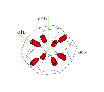
\includegraphics[width=0.4\textwidth]{valleys.eps}  
  \caption{Orientations of the crystal axes and valleys in the lab coordinate system XYZ.}
  \label{fig:valley}
\end{figure}

The dependence of the electron drift velocity $\mathbf{v}_{e}$ on the applied electric field $\mathbf{E}$ is taken to be
\begin{equation}
  \label{eq:ed}
  \mathbf{v}_{e}(\mathbf{E}) = \mathcal{A}(|\mathbf{E}|) \sum_{j} \frac{n_{j}}{n}     \frac{\gamma_{j}\mathbf{E_{0}}}     {\sqrt{\mathbf{E_{0}}\gamma_{j}\mathbf{E_{0}}}},  \mbox{ with }     j=1,2,3,4
\end{equation}
where $\mathcal{A}$ is a function of the magnitude of the electric field and temperature, the value of $\mathcal{A}$ must be negative because electrons drift to the opposite direction of the electric field; $\mathbf{E_{0}}$ is the normalized electric field vector; $n_{j}/n$ is the fraction  of the carriers (in this case, electrons) in the $j$-th $\langle111\rangle$ valley, $\gamma_{j}$ is the effective mass tensor for the $j$-th $\langle111\rangle$ valley. In general the tensor $j$-th is given in terms of the rotation matrices $R_{i}$, responsible for aligning the $j$-th $\langle 111 \rangle$ axis with the Y-axis of the lab system, by
\begin{equation}
  \label{eq:gammas}
  \gamma_{j} = R_{j}^{T}\gamma_{0}R_{j}, \mbox{ with } \gamma_{0}   \equiv \left(
    \begin{array}{ccc}
      m_{t}^{-1} & 0 & 0 \\
      0 & m_{l}^{-1} & 0 \\
      0 & 0 & m_{t}^{-1}
    \end{array} \right),
\end{equation}
where $m_{t} = 1.64m_{e}, m_{l} = 0.0819m_{e}$ with $m_{e}$ denoting the free electron mass, and the rotation matrix $R_{j} = R_{x^{\prime}}(\arccos(\sqrt{2/3}))R_{z}((j-1)\pi/2)$.

\begin{figure}[tbhp]
  \centering
  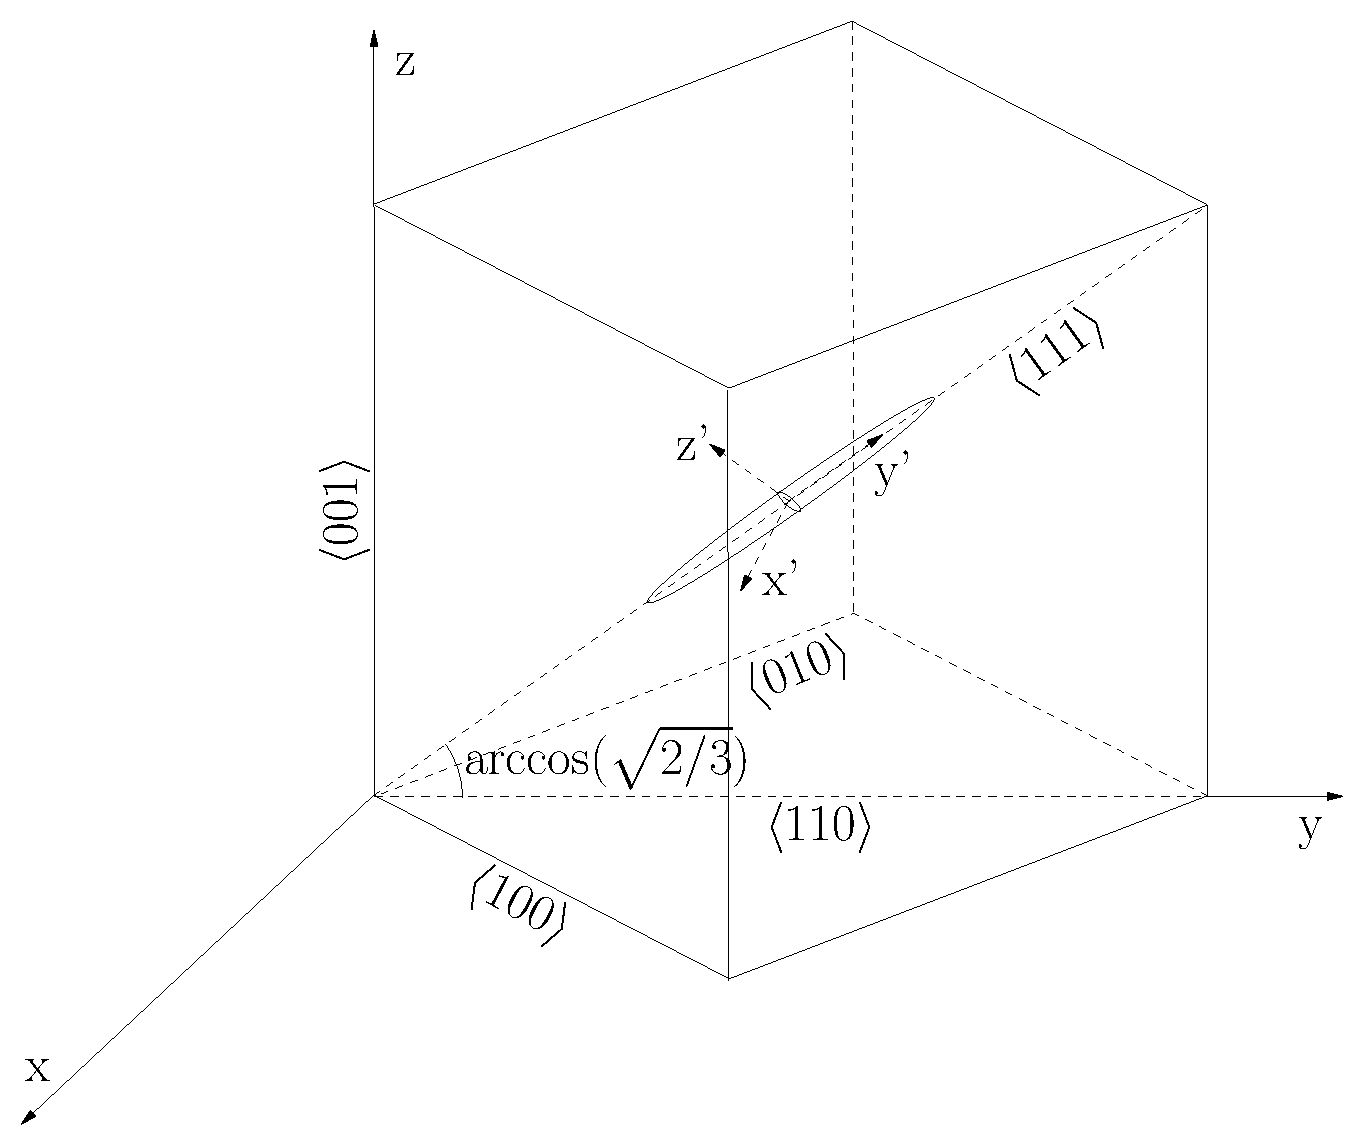
\includegraphics[width=0.6\textwidth]{axes.eps}  
  \caption{Orientations of the crystal axes and valleys in the lab coordinate system XYZ.}
  \label{fig:axes}
\end{figure}

For an experimental determination of the repopulation amplitude, the deviation from a uniform population distribution $n_{e}/n$ (1/4 for germanium) is assumed to vary with the electric field weighted by the factor $\mathcal{R}$:
\begin{equation}
  \label{eq:nion}
  \frac{n_{j}}{n} = \mathcal{R(|\mathbf{E}|)}   \left[         \frac{\sqrt{\mathbf{E_{0}}\gamma_{j}\mathbf{E_{0}}}}
    {\sum_{i}\sqrt{\mathbf{E_{0}}\gamma_{i}\mathbf{E_{0}}}} -               \frac{n_{e}}{n} \right] + \frac{n_{e}}{n},  \mbox{ with }           i=1,2,3,4
\end{equation}

If the electric field vector is equally oriented with respect to all the $\langle111\rangle$ directions, there is an uniform repopulation of the conduction bands, \textit{i.e.} $n_{j}/n = 1/4$. An electric field applied along the $\langle100\rangle$ direction, \textit{i.e.} $\mathbf{E_{0}} = (1/\sqrt{2},1/\sqrt{2},0)^{T}$, satisfies this condition. By employing the experimental drift velocity $v_{e}^{exp}(E)$ for an applied electric field $E$ in the $\langle100\rangle$ direction at a specific temperature, the absolute value  of $\mathcal{A}(|\mathbf{E}|)$ can be calculated as
\begin{equation}
  \label{eq:ae}
  \mathcal{A}(|\mathbf{E}|) = \frac{v_{e}^{exp}(E)}  {\displaystyle \sum_{j}     \frac{1}{4}     \frac{\gamma_{j}\mathbf{E_{0}}}         {\sqrt{\mathbf{E_{0}}\gamma_{j}\mathbf{E_{0}}}} },  \mbox{ with }       \mathbf{E_{0}} = \left( \begin{array}{c} 
    1/\sqrt{2}\\1/\sqrt{2}\\0 \end{array} \right).
\end{equation}

If the electric field vector is oriented along with one of the $\langle111\rangle$ directions, \textit{i.e.} $\mathbf{E_{0}} = (0,\sqrt{2}/\sqrt{3},1/\sqrt{3})^{T}$, there is an uniform repopulation of the conduction bands among the other three $\langle111\rangle$-axes, \textit{i.e.}
\begin{equation}
  \label{eq:n111}
  \frac{n_{2}}{n} = \frac{n_{3}}{n} = \frac{n_{4}}{n}.
\end{equation}
Since
\begin{equation}
  \label{eq:nsum}
  \displaystyle \sum_{j}\frac{n_{j}}{n} = 1,
\end{equation}
we have
\begin{equation}
  \label{eq:n12}
  \frac{n_{1}}{n} + 3\frac{n_{2}}{n}= 1.
\end{equation}
By employing the experimental drift velocity $v_{e}^{exp}(E)$ for an applied electric field $E$ in the $\langle111\rangle$ direction at a specific temperature, we have another relation between $n_{1}/n$ and $n_{2}/n$:
\begin{equation}
  \label{eq:n12p}
  v_{e}^{exp}(E) =  \mathcal{A}(|\mathbf{E}|) \left(  \frac{n_{1}}{n} \frac{\gamma_{1}\mathbf{E_{0}}}         {\sqrt{\mathbf{E_{0}}\gamma_{1}\mathbf{E_{0}}}} +  3\frac{n_{2}}{n} \frac{\gamma_{2}\mathbf{E_{0}}}         {\sqrt{\mathbf{E_{0}}\gamma_{2}\mathbf{E_{0}}}} \right).
\end{equation}
One can get the value of $n_{1}/n$ and $n_{2}/n$ by solving the equations \ref{eq:n12} and \ref{eq:n12p} together. Then $\mathcal{R}(|\mathbf{E}|)$ can be calculated as
\begin{equation}
  \label{eq:re}
  \mathcal{R(|\mathbf{E}|)} = \left( \frac{n_{1}}{n} - \frac{n_{e}}{n}     \right) / \left(     \frac{\sqrt{\mathbf{E_{0}}\gamma_{1}\mathbf{E_{0}}}}
    {\sum_{i}\sqrt{\mathbf{E_{0}}\gamma_{i}\mathbf{E_{0}}}} -                           \frac{n_{e}}{n} \right),  \mbox{ with }           i=1,2,3,4 \mbox{ and       } \mathbf{E_{0}} = \left( \begin{array}{c} 
      0\\ \sqrt{2/3}\\\sqrt{1/3} \end{array} \right).
\end{equation}

The dependence of the experimental $\langle111\rangle$ and $\langle100\rangle$ drift velocities on the electric field can be calculated using Eq.~\ref{eq:para}. After determination of the parameters $\mathcal{A}$ and $\mathcal{R}$, the drift velocity can be calculated for any direction and any strength of the electric field.

\subsubsection{Hole drift velocity}
\label{sec:hole}
The three components $(v_{x^{\prime}}, v_{y^{\prime}}, v_{z^{\prime}})^{T}$ of the hole drift velocity $\mathbf{v}$ in the local coordinate $x^{\prime}y^{\prime}z^{\prime}$ (as shown in Fig.~\ref{fig:vsphere}) can be expressed as:
\begin{equation}
  \label{eq:vsphere}
  \begin{array}{rcl}
   v_{x^{\prime}} = v_{r} &=& v_{100}(E)[1-\Lambda(k_{0})(\sin(\theta)^{4}\sin(2\phi)^{2} + \sin(2\theta)^{2})]\\
   v_{y^{\prime}} = v_{\theta} &=& v_{100}(E)\Omega(k_{0})[2\sin(\theta)^{3}\cos(\theta)\sin(2\phi)^{2} + \sin(4\theta)]\\
    v_{z^{\prime}} = v_{\phi} &=& v_{100}(E)\Omega(k_{0})\sin(\theta)^{3}\sin(4\phi)
  \end{array}
\end{equation}
\begin{figure}[tbhp]
  \centering
  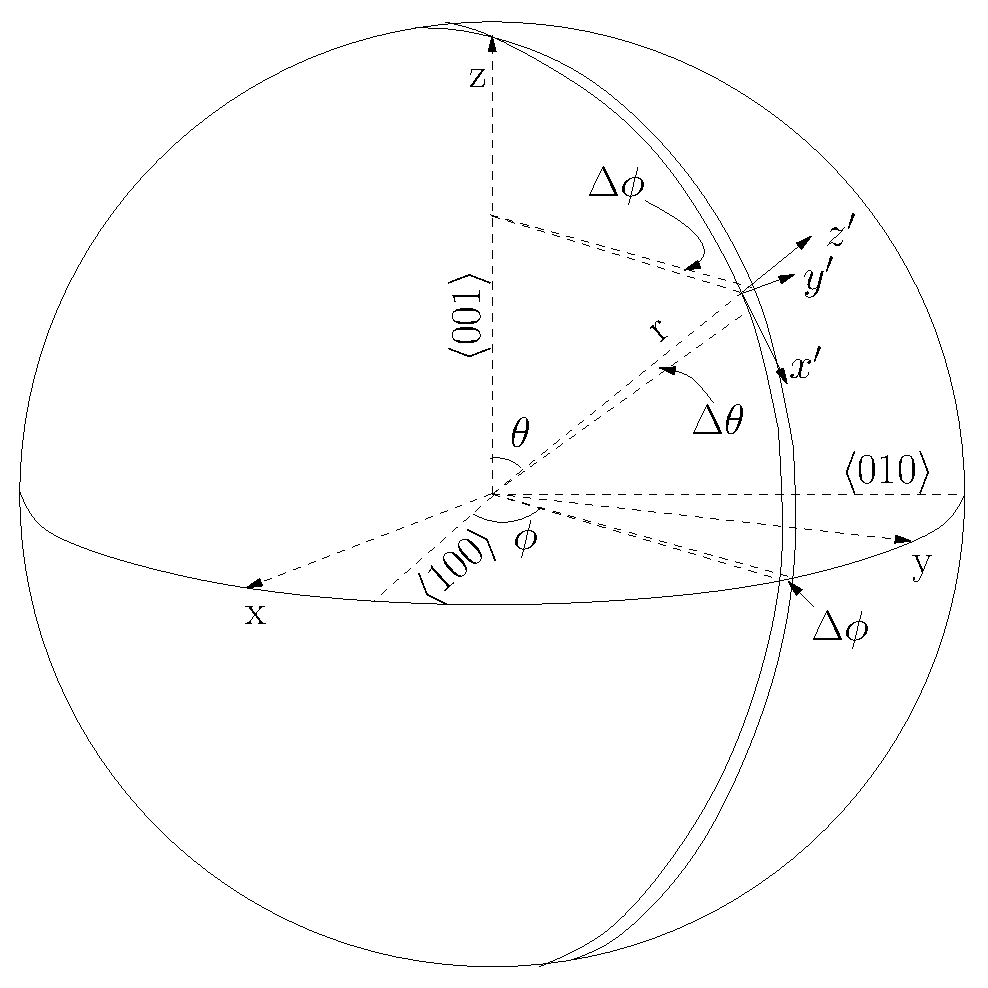
\includegraphics[width=0.6\textwidth]{vsphere.eps}  
  \caption{Orientations of the crystal axes and valleys in the lab
coordinate system XYZ.}
  \label{fig:vsphere}
\end{figure}
The mean wave number $k_{0}$ can be expressed as a function of $v_{rel} = v_{111}/v_{100}$:
\begin{equation}
  \label{eq:k0}
   k_{0}(v_{rel}) = 9.2652 - 26.3467v_{rel} + 29.6137v_{rel}^{2} - 12.3689v_{rel}^{3}
\end{equation}
The function $\Lambda$ and $\Omega$ govern the amplitude of the anisotropy and can be expressed as
\begin{equation}
  \label{eq:lamb}
   \Lambda(k_{0}) = -0.01322k_{0} + 0.41145k_{0}^{2} - 0.23657k_{0}^{3} + 0.04077k_{0}^{4}
\end{equation}
\begin{equation}
  \label{eq:ome}
   \Omega(k_{0}) = 0.006550k_{0} - 0.19946k_{0}^{2} + 0.09859k_{0}^{3} - 0.01559k_{0}^{4}
\end{equation}
The dependence of the experimental $\langle111\rangle$ and $\langle100\rangle$ drift velocities, \textit{i.e.} $v_{111}$ and $v_{100}$ on the electric field can be calculated using Eq.~\ref{eq:para}.

The three components $(v_{x}, v_{y}, v_{z})^{T}$ of the hole drift velocity $\mathbf{v}$ in the lab coordinate $xyz$ (as shown in Fig.~\ref{fig:vsphere}) can be calculated as:
\begin{equation}
  \label{eq:v2v}  
  \left(
    \begin{array}{c}
      v_{x} \\ v_{y} \\ v_{z}
    \end{array}
\right) = R_{z}(\phi + \frac{\pi}{4} + \phi_{110}) R_{y^{\prime}}(\theta) \left( 
    \begin{array}{c}
      v_{x^{\prime}} \\ v_{y^{\prime}} \\ v_{z^{\prime}}
    \end{array} \right)
\end{equation}

%%% Local Variables:
%%% mode:latex
%%% TeX-master: "GSTR-08-M007"
%%% End:
